\chapter{Result}
104 Borehole Log Data of 31 locations inside Kathmandu and Lalitpur district areas were taken into consideration. The results were obtained after calculating Bearing Capacity at 1.5m, 3m, and 4.5m depth by shear criteria using Terzaghi, Meyerhof, Hansen, Vesic and Teng methods and Plaxis2D software and by deflection criteria using Bowels, Teng, Peck, Meyerhof  methods and Plaxis2D software. The median value of those methods are taken and mapped for those depths. Liquifaction Potential Index of the area is also mapped.
\pagebreak

\section{Location Table}
\begin{table}[!h]
\caption{Location Table}
\begin{tabularx}{\textwidth}{ | l | p{0.6\textwidth} | X | X | }
\hline
 \textbf{S.N.} & \textbf{Location} & \textbf{Latitude} & \textbf{Longitude} \\
\hline
 1 & Rastriya Banijya Bank: Thapathali, Kathmandu & 27.65586 & 85.30645 \\
 2 & Building Complex: Anamnagar, Kathmandu & 27.69728 & 85.32746 \\
 3 & Building Complex: Bakhundol Lalitpur & 27.68302 & 85.31033 \\
 4 & Hindu vidhypeth: Balkumari, Lalitpur & 27.67114 & 85.33793 \\
 5 & DI Skin Health and Referral Center (P). Ltd.: Bansbari, Kathmandu & 27.73704 & 85.33354 \\
 6 & Building: Bhaisipati, Lalitpur & 27.64805 & 85.29596 \\
 7 & Brihaspati Vidyasadan School: Gahanapokhari, Kathmandu & 27.71425 & 85.32957 \\
 8 & Green Hill City (P). Ltd. : Mulpani, Kathamndu  & 27.71577 & 85.38647 \\
 9 & Building Site: Itachhe tol, Bhaktapur & 27.67284 & 85.42261 \\
 10 & Buddha Air (P). Ltd. : Jawalakhel, Lalitpur  & 27.67357 & 85.31187 \\
 11 & Tamrakar Samaj: Jawalakhel & 27.67475 & 85.31220 \\
 12 & Tangal, Kathmandu & 27.72009 & 85.32626 \\
 13 & Harihar Bhavan, Lalitpur & 27.68047 & 85.31111 \\
 14 & Janamaitri Campus: Kuleswore, Kathmandu & 27.69173 & 85.29005 \\
 15 & Amrit Science Campus: Lainchour, Kathmandu & 27.71776 & 85.31061 \\
 16 & Mahendra Ratna Campus: Tahachal, Kathmandu & 27.70346 & 85.29821 \\
 17 & Bhatbhateni Supermarket \& Departmental Store: Satdobato, Lalitpur & 27.65712 & 85.32002 \\
 18 & Nepal Mountaineering Association :  Naxal, Nagpokhari Kathmandu  & 27.71303 & 85.32167 \\
 19 & Patanjali Yogpeeth Nepal : Mandikatar, Kathmandu  & 27.74115 & 85.34555 \\
 20 & Mandikhatar, Kathmandu  & 27.73878 & 85.34535 \\
 21 & CIWEC Clinic: Lainchaur, Kathmandu  & 27.72040 & 85.31555 \\
 22 & Vastukala Pharamarsha Nepal : Kupondole, Lalitpur & 27.68376 & 85.31634 \\
 23 & Building: Kupondole, Lalitpur & 27.68628 & 85.31470 \\
 24 & NAST Technology : Khumaltar, Lalitpur & 27.65610 & 85.32768 \\
 25 & Building: Khumaltar, Lalitpur  & 27.64870 & 85.32034 \\
 26 & Building: Kalopul, Pumori, Kathmandu & 27.71183 & 85.33536 \\
 27 & Building Site : Gwarkho, Lalitpur & 27.66601 & 85.32847 \\
 28 & Building: Kumaripati, Lalitpur & 27.67025 & 85.31863 \\
 29 & Building: Kupandole, Lalitpur & 27.68703 & 85.30930 \\
 30 & Nepal Rastra Bank: Thapathali & 27.69023 & 85.31993 \\
 31 & Exam Mega Hall Construction Project : Kirtipur, Kathmandu & 27.68426 & 85.29536 \\
\hline
\end{tabularx}

\end{table}
\pagebreak

\section{Locations map\index{map}}
\begin{figure}[!hbt]
\centering
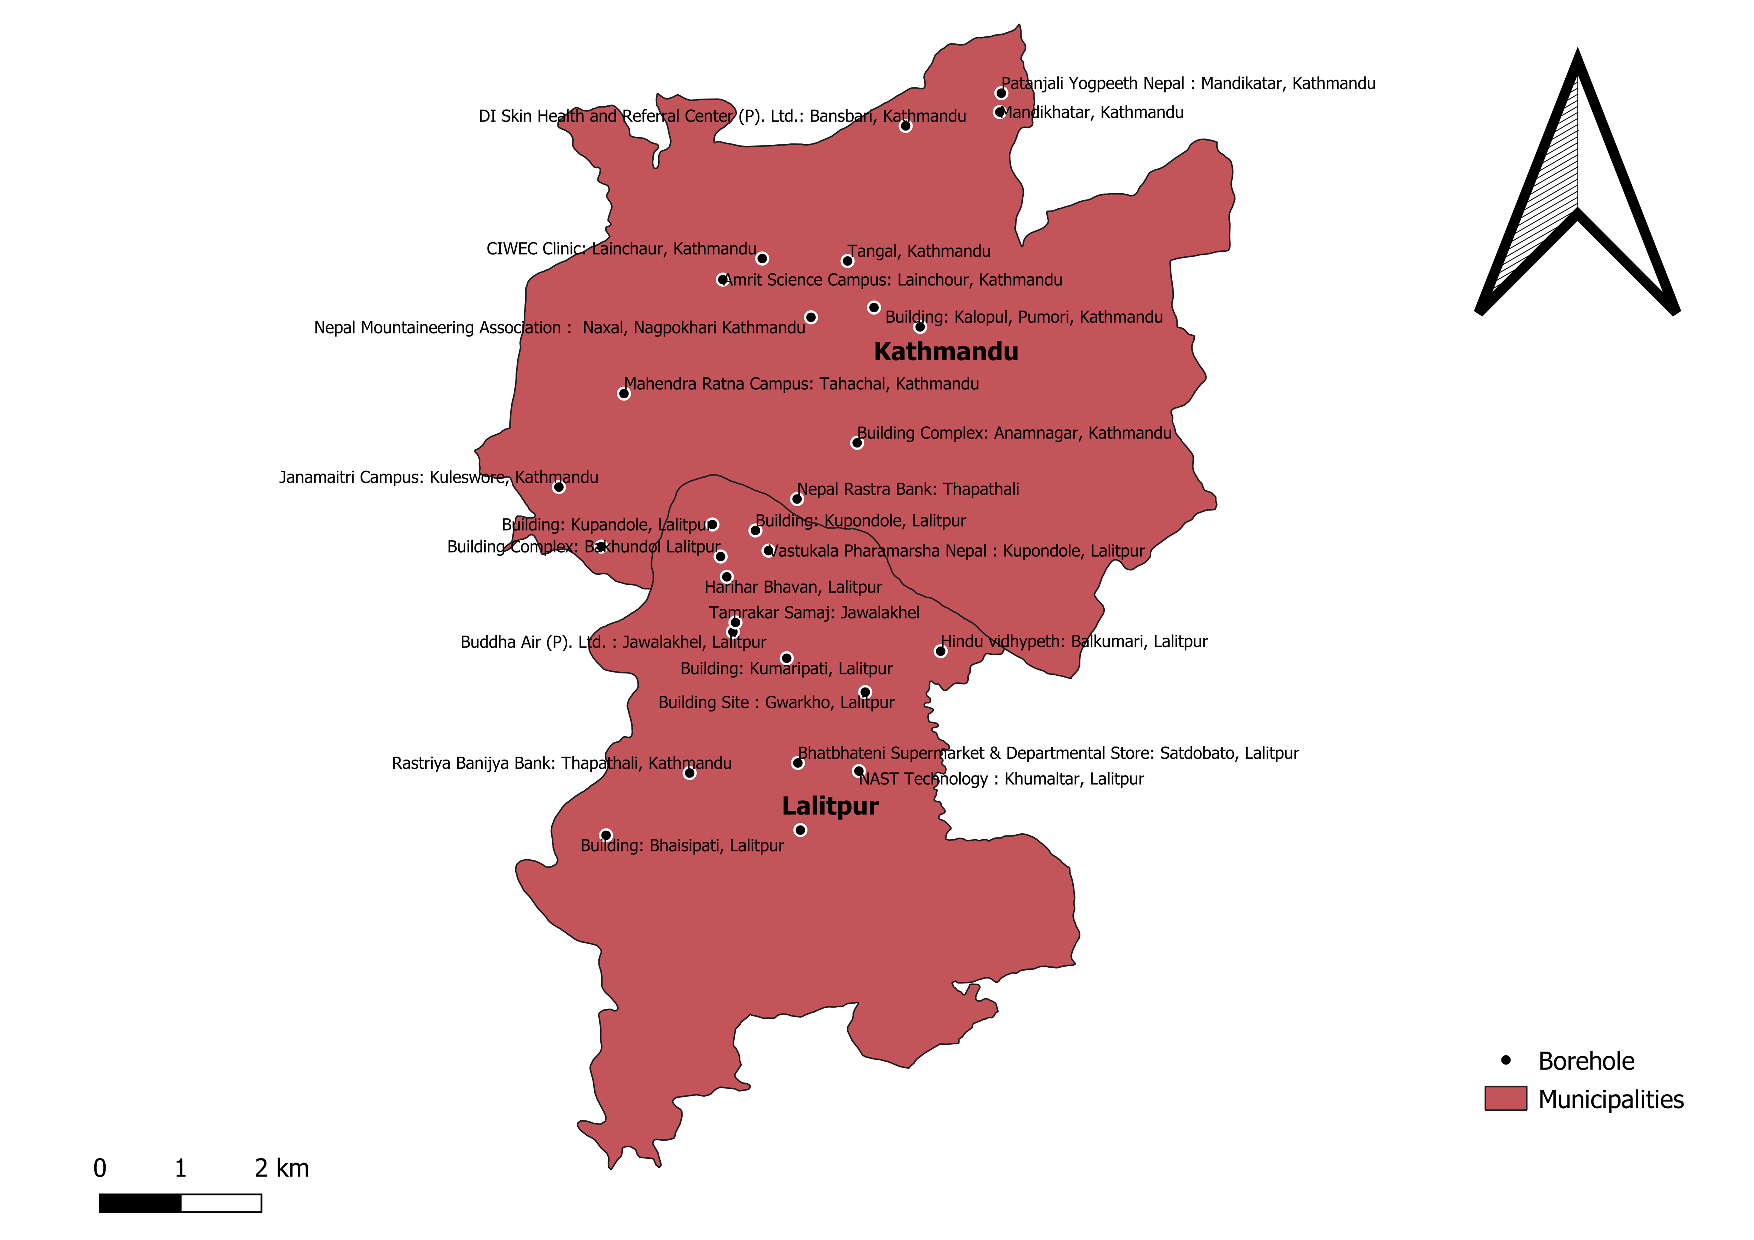
\includegraphics[width=\linewidth, height=\textheight,keepaspectratio]{in/map/Borehole2.png}
\caption{Borehole locations\index{map}}
\end{figure}
\pagebreak

\section{Shear Strength Table(KPa)}
\begin{table}[!h]
\caption{Shear Strength Table}
\begin{tabularx}{\textwidth}{ | l | p{0.5\textwidth} | X | X | X | }
\hline
 \textbf{S.N.} & \textbf{Location} & \textbf{1.5m} & \textbf{3.0m} & \textbf{4.5m}\\
\hline
 1 & Thapathali, Kathmandu & 556.783 & 881.966 & 1219.911 \\
 2 & Anamnagar, Kathmandu & 226.203 & 253.102 & 210.010 \\
 3 & Bakhundol Lalitpur & 78.274 & 109.557 & 126.082 \\
 4 & Balkumari, Lalitpur & 347.149 & 705.395 & 497.897 \\
 5 & Bansbari, Kathmandu & 226.203 & 411.124 & 573.964 \\
 6 & Bhaisipati, Lalitpur & 318.034 & 654.486 & 375.495 \\
 7 & Gahanapokhari, Kathmandu & 160.596 & 211.665 & 408.875 \\
 8 & Mulpani, Kathamndu  & 85.764 & 155.830 & 738.492 \\
 9 & Itachhe tol, Bhaktapur & 103.915 & 141.288 & 161.811 \\
 10 & Jawalakhel, Lalitpur  & 295.379 & 525.479 & 351.012 \\
 11 & Jawalakhel & 154.538 & 188.042 & 218.952 \\
 12 & Tangal, Kathmandu & 818.280 & 1500.181 & 1701.000 \\
 13 & Harihar Bhavan, Lalitpur & 678.380 & 862.325 & 1080.162 \\
 14 & Kuleswore, Kathmandu & 258.687 & 440.825 & 510.316 \\
 15 & Lainchour, Kathmandu & 427.627 & 1031.251 & 1534.093 \\
 16 & Tahachal, Kathmandu & 213.742 & 278.658 & 324.310 \\
 17 & Satdobato, Lalitpur & 664.956 & 750.835 & 216.900 \\
 18 & Naxal, Nagpokhari Kathmandu  & 661.987 & 1034.337 & 1088.942 \\
 19 & Mandikatar, Kathmandu  & 216.255 & 558.979 & 750.723 \\
 20 & Mandikhatar, Kathmandu  & 166.394 & 374.942 & 819.365 \\
 21 & Lainchaur, Kathmandu  & 961.112 & 1349.100 & 1269.905 \\
 22 & Kupondole, Lalitpur & 197.198 & 707.709 & 1129.132 \\
 23 & Kupondole, Lalitpur & 177.101 & 213.827 & 248.214 \\
 24 & Khumaltar, Lalitpur & 130.857 & 158.837 & 179.932 \\
 25 & Khumaltar, Lalitpur  & 113.986 & 140.911 & 169.485 \\
 26 & Kalopul, Pumori, Kathmandu & 702.484 & 1078.437 & 1160.662 \\
 27 & Gwarkho, Lalitpur & 101.891 & 139.931 & 175.822 \\
 28 & Kumaripati, Lalitpur & 976.011 & 1705.445 & 1978.329 \\
 29 & Kupandole, Lalitpur & 107.883 & 127.698 & 152.281 \\
 30 & Thapathali & 381.822 & 577.350 & 761.849 \\
 31 & Kirtipur, Kathmandu & 363.008 & 713.392 & 1008.880 \\
\hline
\multicolumn{2}{|X|}{\mbox{Mean($\overline{x}$)}} & 350.726 & 580.094 & 682.026 \\
\multicolumn{2}{|X|}{\mbox{Standard deviation($\sigma$)}} & 262.236 & 428.627 & 505.678 \\
\multicolumn{2}{|X|}{\mbox{Minimum($x_{min}$)}} & 78.274 & 109.557 & 126.082 \\
\multicolumn{2}{|X|}{\mbox{Maximum($x_{max}$)}} & 976.011 & 1705.445 & 1978.329 \\
\hline
\end{tabularx}

\end{table}
\pagebreak

\section{1.5m Bearing Capacity(shear)\index{map}}
\begin{figure}[!hbt]
\centering
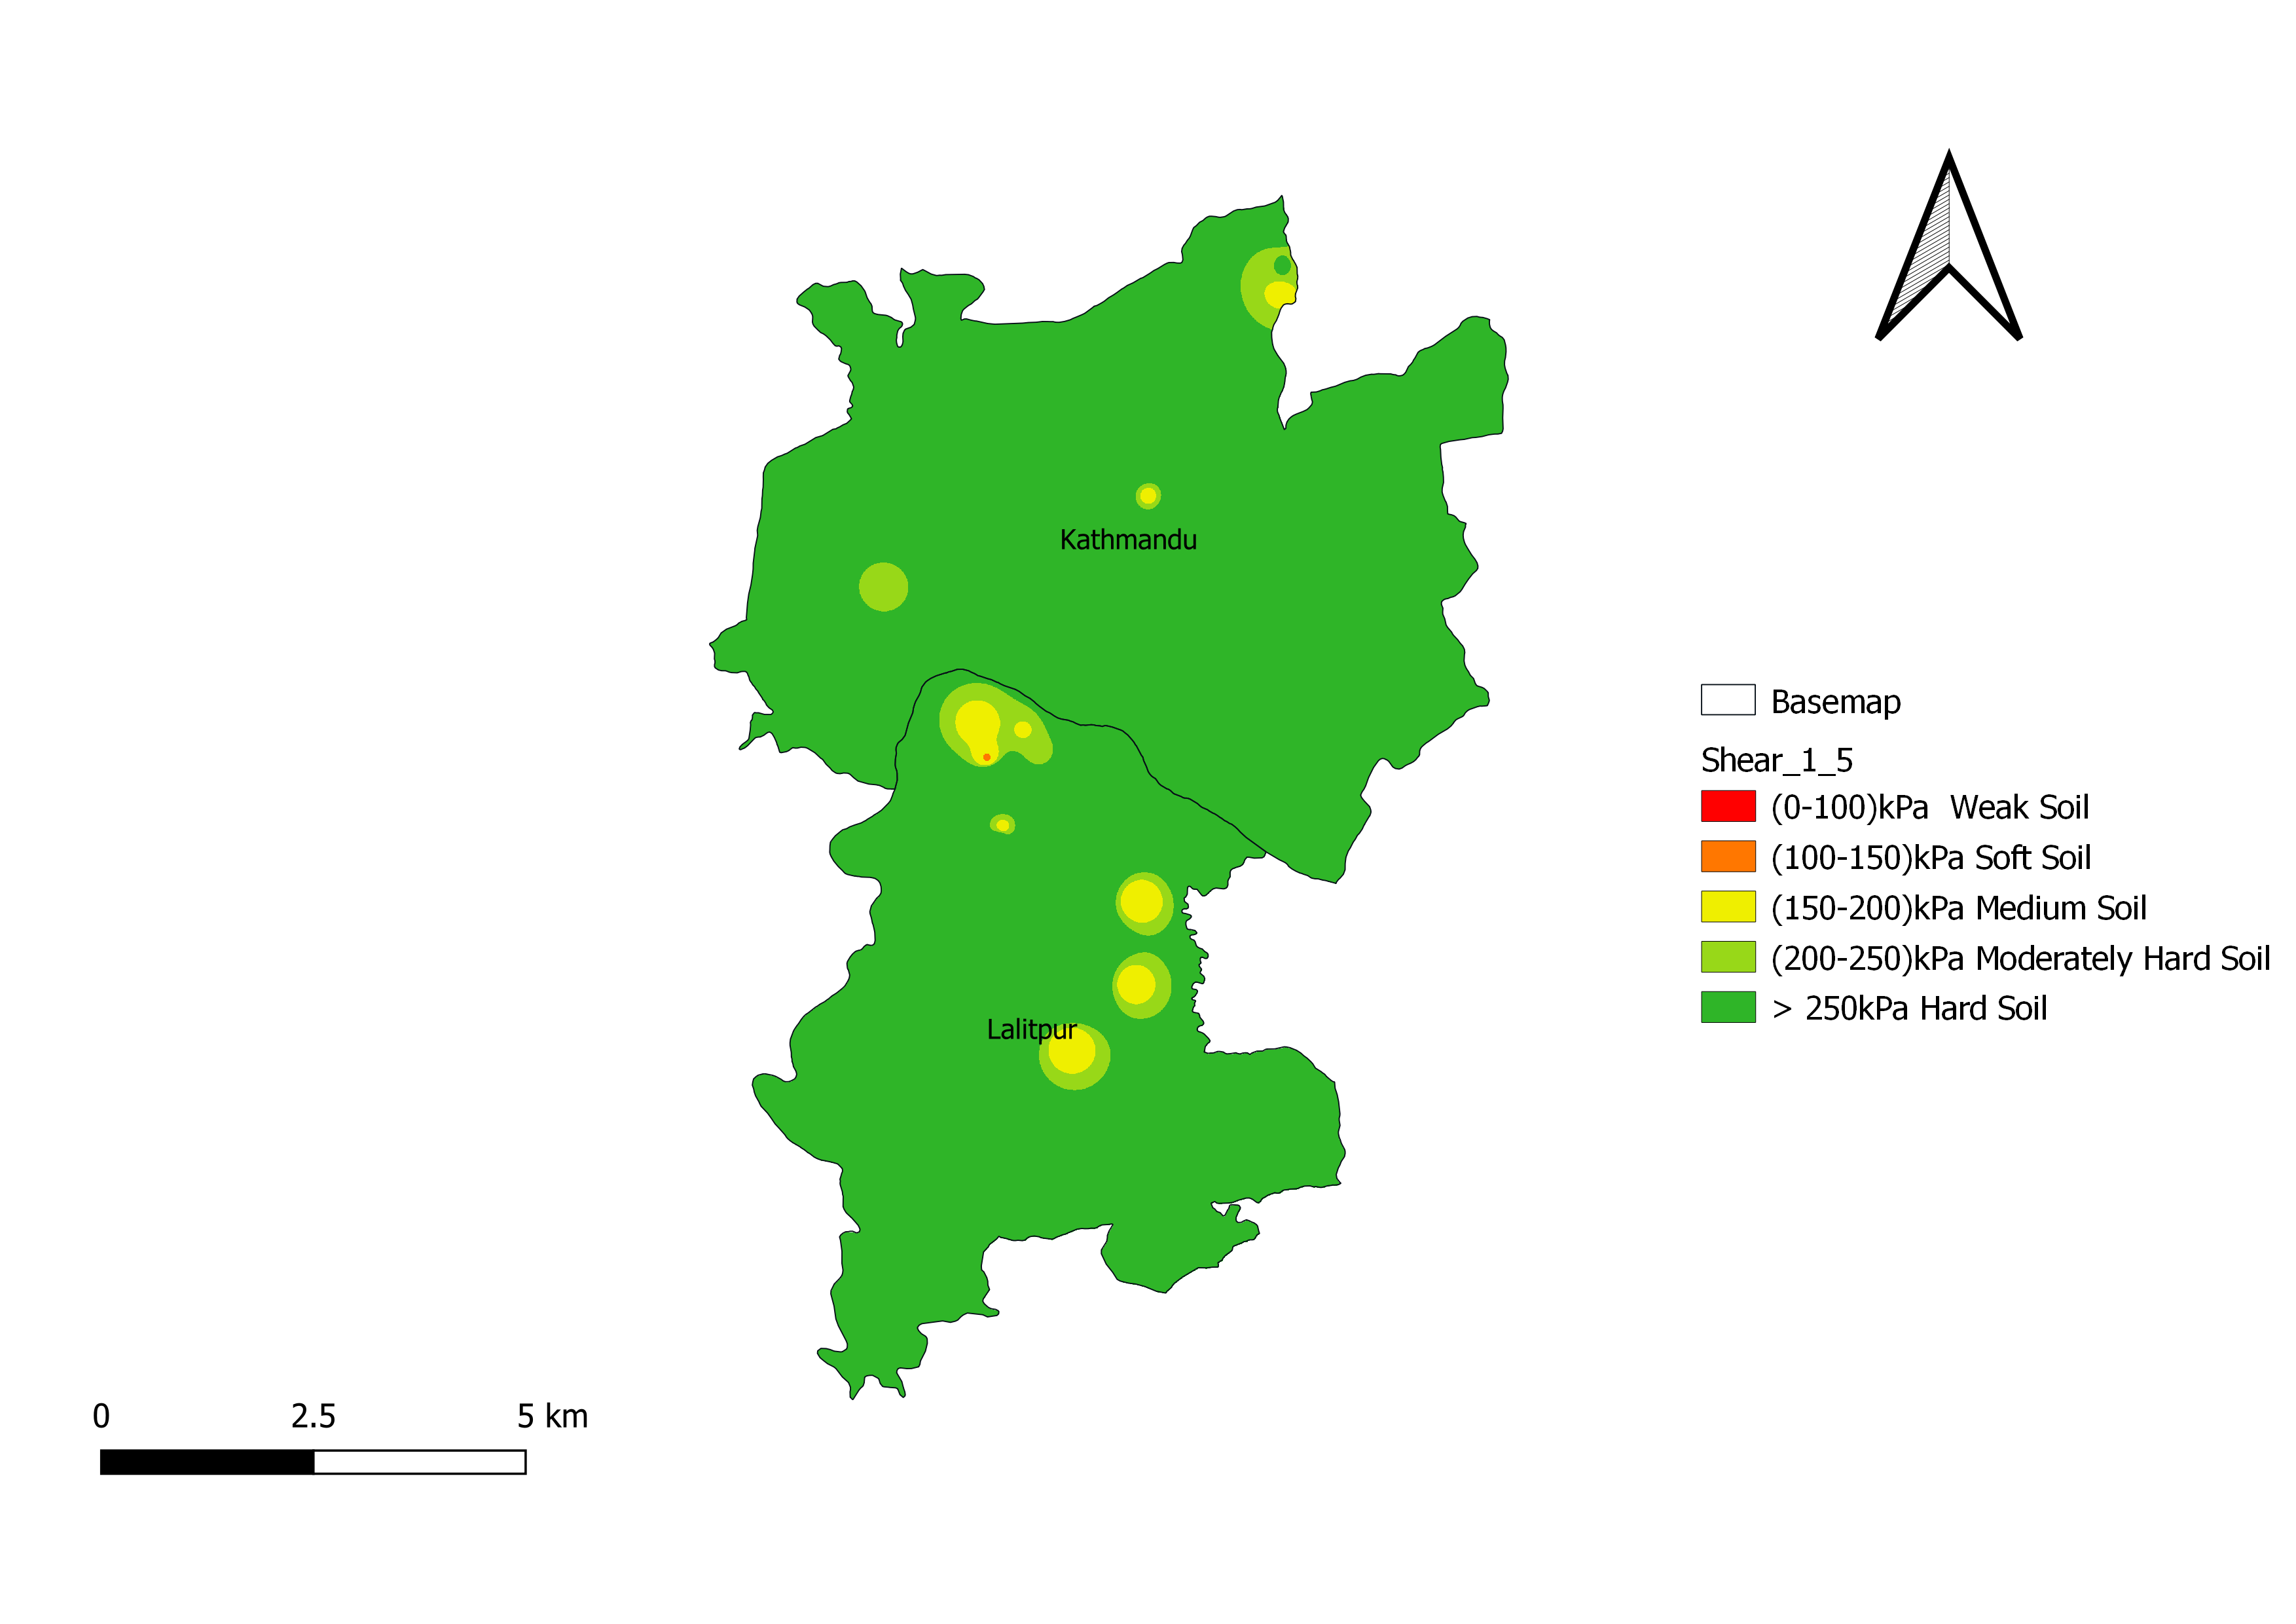
\includegraphics[width=\linewidth, height=\textheight,keepaspectratio]{in/map/Shear_1_5.png}
\caption{BC at 1.5m depth}
\end{figure}
\pagebreak

\section{3.0m Bearing Capacity(shear)\index{map}}
\begin{figure}[!hbt]
\centering
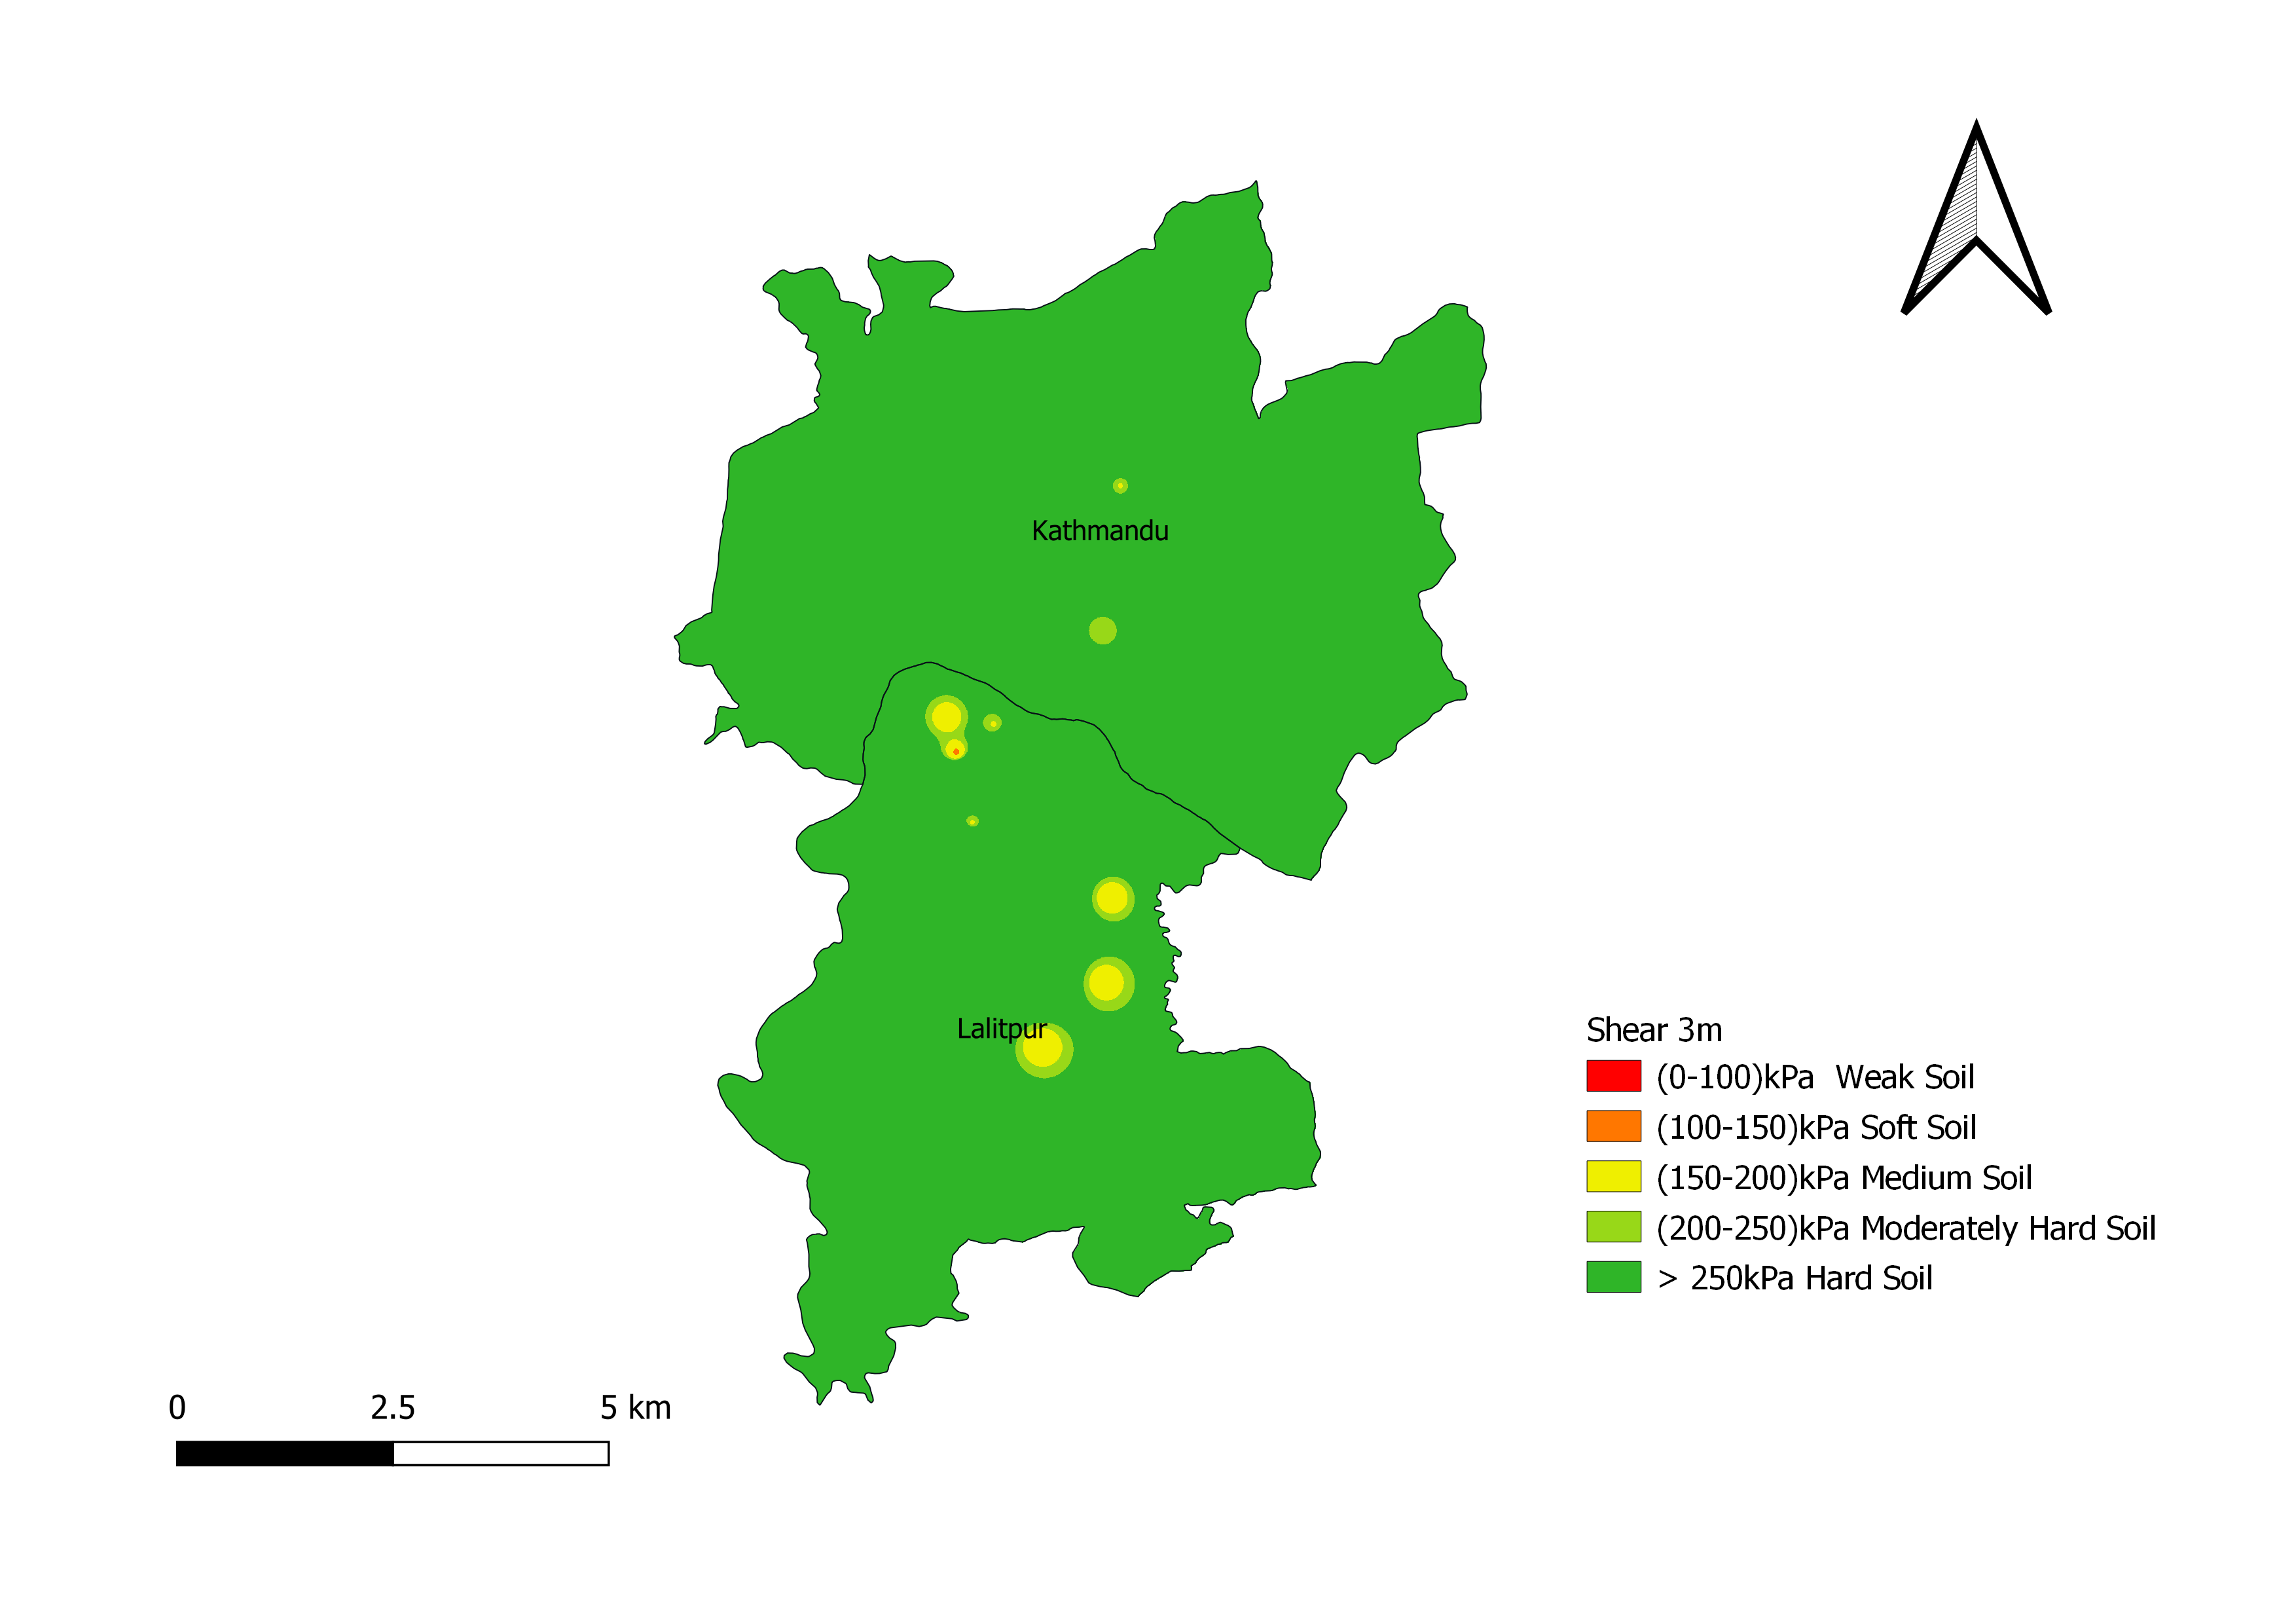
\includegraphics[width=\linewidth, height=\textheight,keepaspectratio]{in/map/Shear_3_0.png}
\caption{BC at 3.0m depth}
\end{figure}
\pagebreak

\section{4.5m Bearing Capacity(shear)\index{map}}
\begin{figure}[!hbt]
\centering
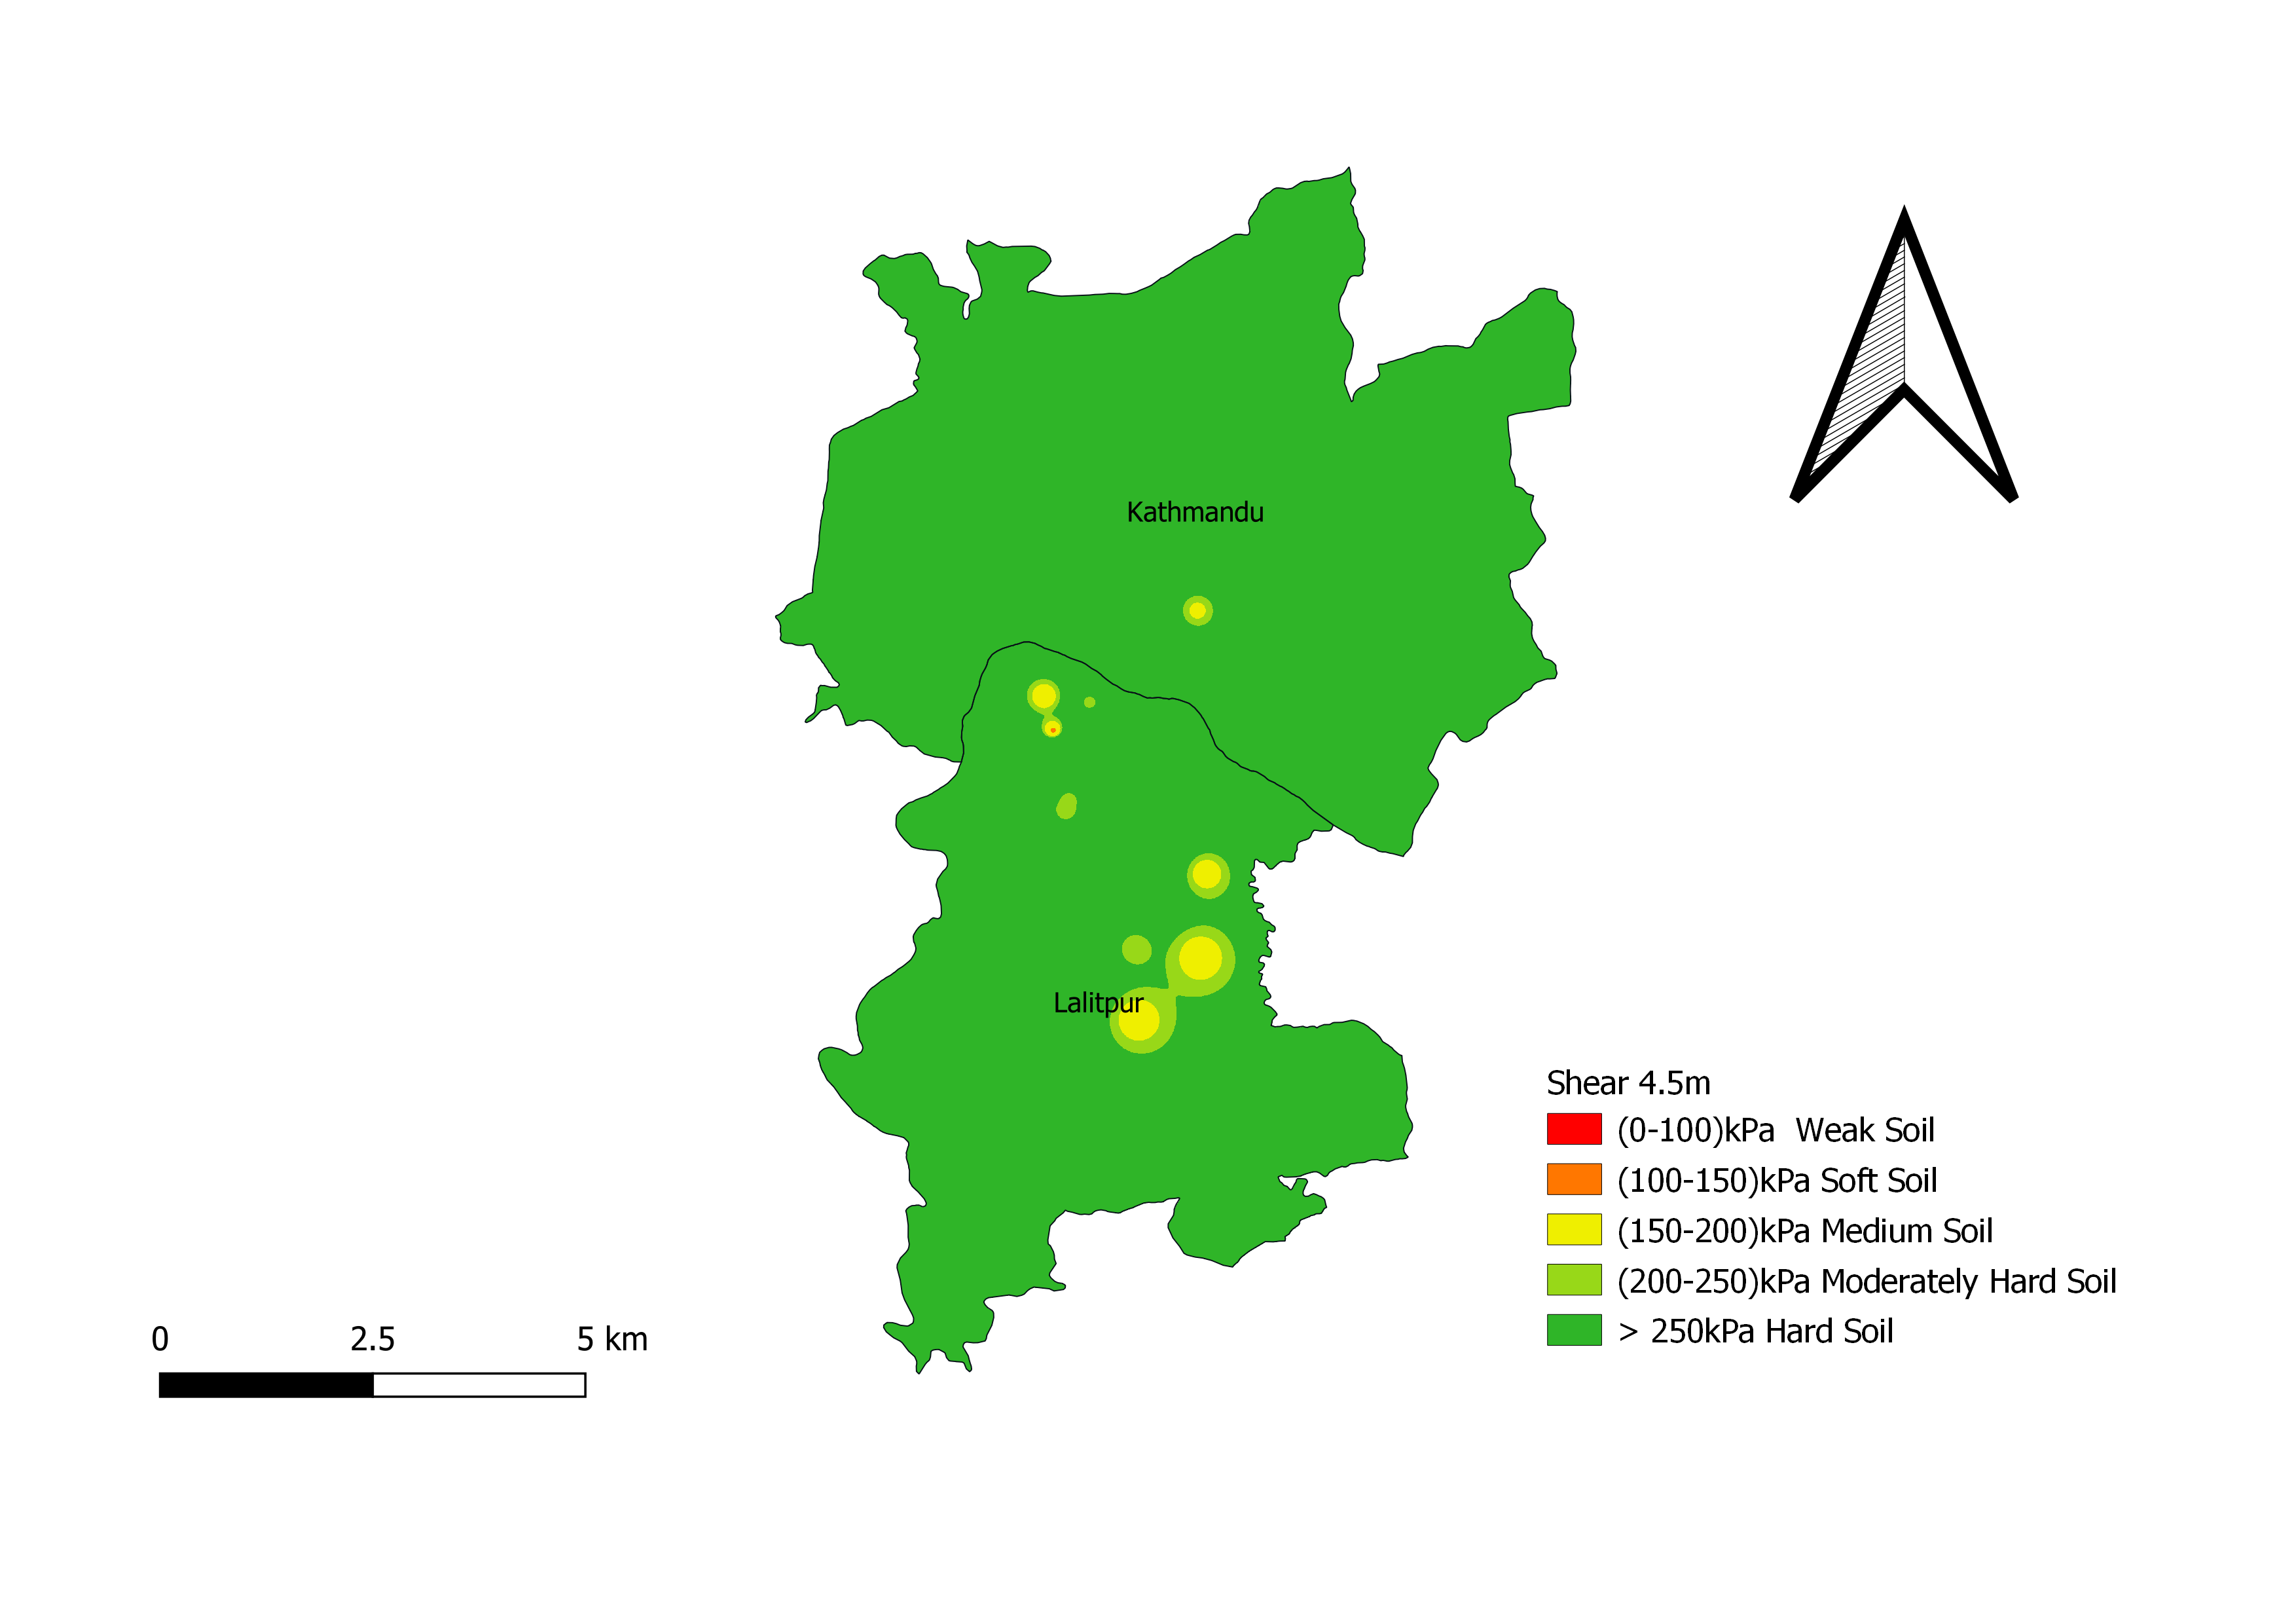
\includegraphics[width=\linewidth, height=\textheight,keepaspectratio]{in/map/Shear_4_5.png}
\caption{BC at 4.5m depth}
\end{figure}
\pagebreak

\section{Settlement Strength Table(KPa, for 25mm)}
\begin{table}[!h]
\caption{Settlement Strength Table}
\begin{tabularx}{\textwidth}{ | l | p{0.5\textwidth} | X | X | X | }
\hline
 \textbf{S.N.} & \textbf{Location} & \textbf{1.5m} & \textbf{3.0m} & \textbf{4.5m}\\
\hline
 1 & Thapathali, Kathmandu & 32.327 & 38.642 & 50.943 \\
 2 & Anamnagar, Kathmandu & 178.573 & 98.242 & 71.612 \\
 3 & Bakhundol Lalitpur & 44.627 & 44.584 & 45.737 \\
 4 & Balkumari, Lalitpur & 277.689 & 199.590 & 138.268 \\
 5 & Bansbari, Kathmandu & 143.756 & 135.484 & 150.310 \\
 6 & Bhaisipati, Lalitpur & 310.341 & 303.309 & 200.444 \\
 7 & Gahanapokhari, Kathmandu & 145.774 & 155.979 & 145.323 \\
 8 & Mulpani, Kathamndu  & 65.598 & 120.769 & 182.885 \\
 9 & Itachhe tol, Bhaktapur & 71.789 & 74.786 & 83.443 \\
 10 & Jawalakhel, Lalitpur  & 371.723 & 312.830 & 175.017 \\
 11 & Jawalakhel & 226.421 & 359.938 & 174.803 \\
 12 & Tangal, Kathmandu & 174.929 & 133.731 & 129.194 \\
 13 & Harihar Bhavan, Lalitpur & 43.732 & 41.417 & 39.361 \\
 14 & Kuleswore, Kathmandu & 91.046 & 66.566 & 50.069 \\
 15 & Lainchour, Kathmandu & 182.240 & 245.151 & 236.805 \\
 16 & Tahachal, Kathmandu & 43.164 & 60.422 & 72.989 \\
 17 & Satdobato, Lalitpur & 510.209 & 252.241 & 144.841 \\
 18 & Naxal, Nagpokhari Kathmandu  & 73.785 & 85.657 & 108.810 \\
 19 & Mandikatar, Kathmandu  & 248.511 & 248.768 & 168.528 \\
 20 & Mandikhatar, Kathmandu  & 127.783 & 266.774 & 281.543 \\
 21 & Lainchaur, Kathmandu  & 174.929 & 181.025 & 188.245 \\
 22 & Kupondole, Lalitpur & 248.511 & 319.444 & 341.663 \\
 23 & Kupondole, Lalitpur & 143.756 & 104.626 & 97.679 \\
 24 & Khumaltar, Lalitpur & 133.930 & 60.043 & 48.454 \\
 25 & Khumaltar, Lalitpur  & 109.923 & 101.519 & 83.482 \\
 26 & Kalopul, Pumori, Kathmandu & 119.431 & 112.012 & 101.643 \\
 27 & Gwarkho, Lalitpur & 76.146 & 76.876 & 62.440 \\
 28 & Kumaripati, Lalitpur & 606.172 & 523.712 & 466.218 \\
 29 & Kupandole, Lalitpur & 53.935 & 50.015 & 49.253 \\
 30 & Thapathali & 105.779 & 85.681 & 77.141 \\
 31 & Kirtipur, Kathmandu & 103.824 & 89.948 & 65.702 \\
\hline
\multicolumn{2}{|X|}{\mbox{Mean($\overline{x}$)}} & 142.206 & 147.536 & 118.102 \\
\multicolumn{2}{|X|}{\mbox{Standard deviation($\sigma$)}} & 85.117 & 94.886 & 62.637 \\
\multicolumn{2}{|X|}{\mbox{Minimum($x_{min}$)}} & 32.327 & 38.642 & 39.361 \\
\multicolumn{2}{|X|}{\mbox{Maximum($x_{max}$)}} & 371.723 & 359.938 & 281.543 \\
\hline
\end{tabularx}

\end{table}
\pagebreak

\section{1.5m Bearing Capacity(settlement)\index{map}}
\begin{figure}[!hbt]
\centering
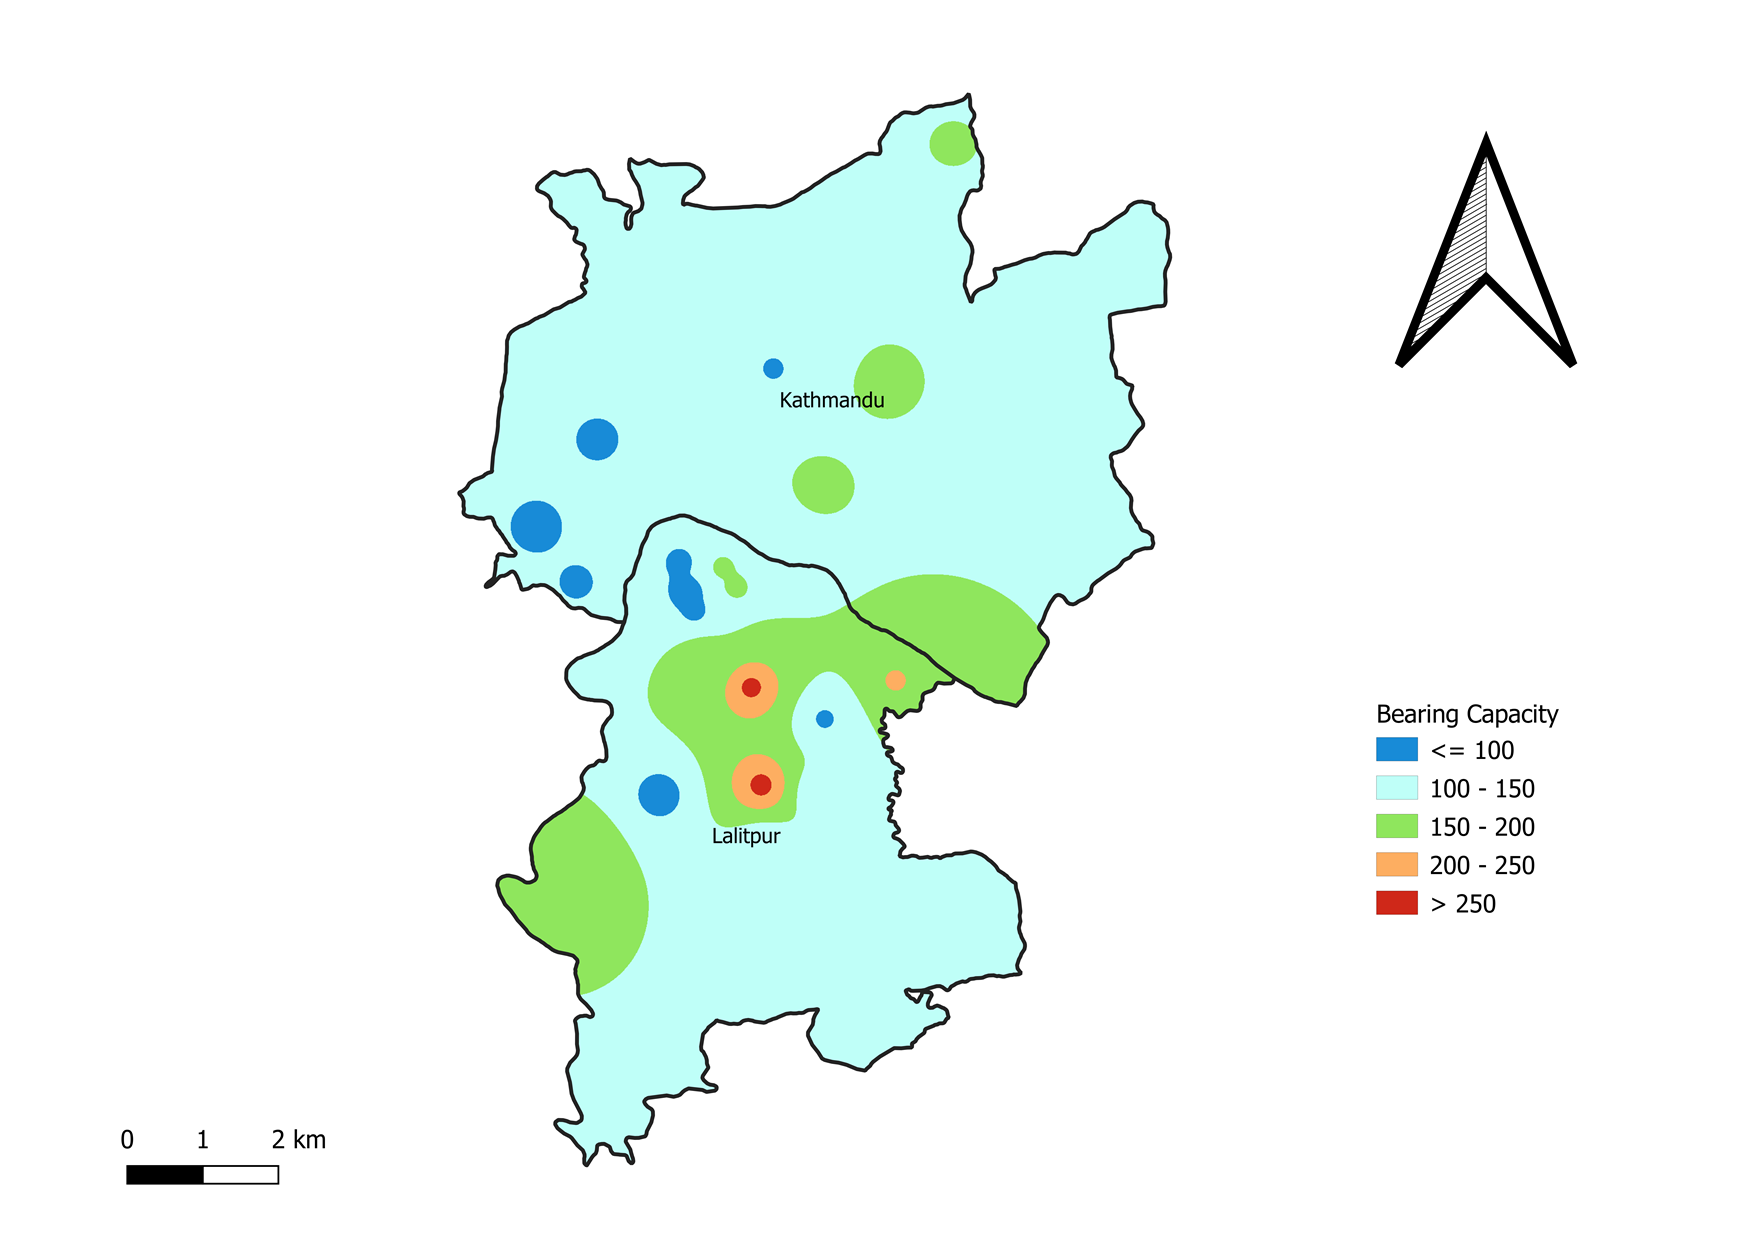
\includegraphics[width=\linewidth, height=\textheight,keepaspectratio]{in/map/Deflection_1_5.png}
\caption{BC at 1.5m depth}
\end{figure}
\pagebreak

\section{3.0m Bearing Capacity(settlement)\index{map}}
\begin{figure}[!hbt]
\centering
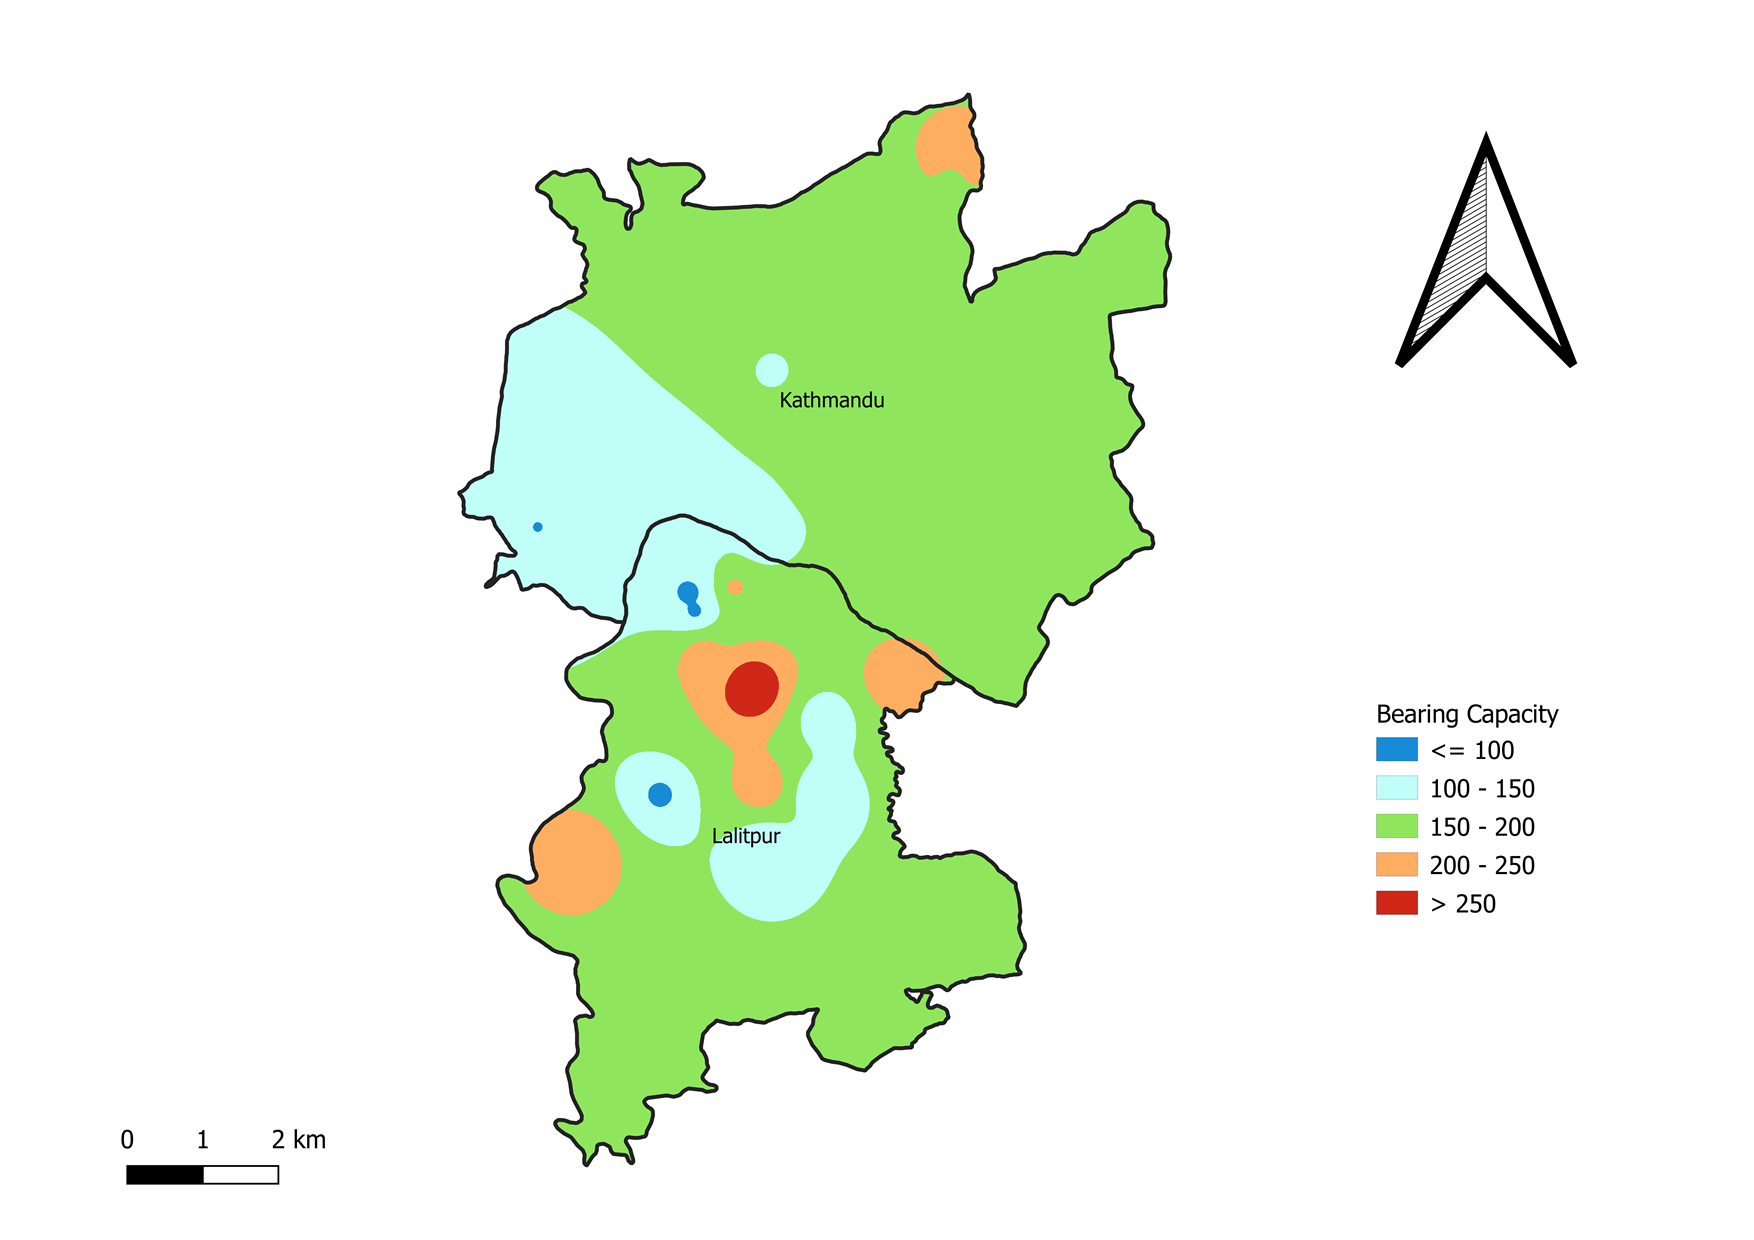
\includegraphics[width=\linewidth, height=\textheight,keepaspectratio]{in/map/Deflection_3_0.png}
\caption{BC at 3.0m depth}
\end{figure}
\pagebreak

\section{4.5m Bearing Capacity(settlement)\index{map}}
\begin{figure}[!hbt]
\centering
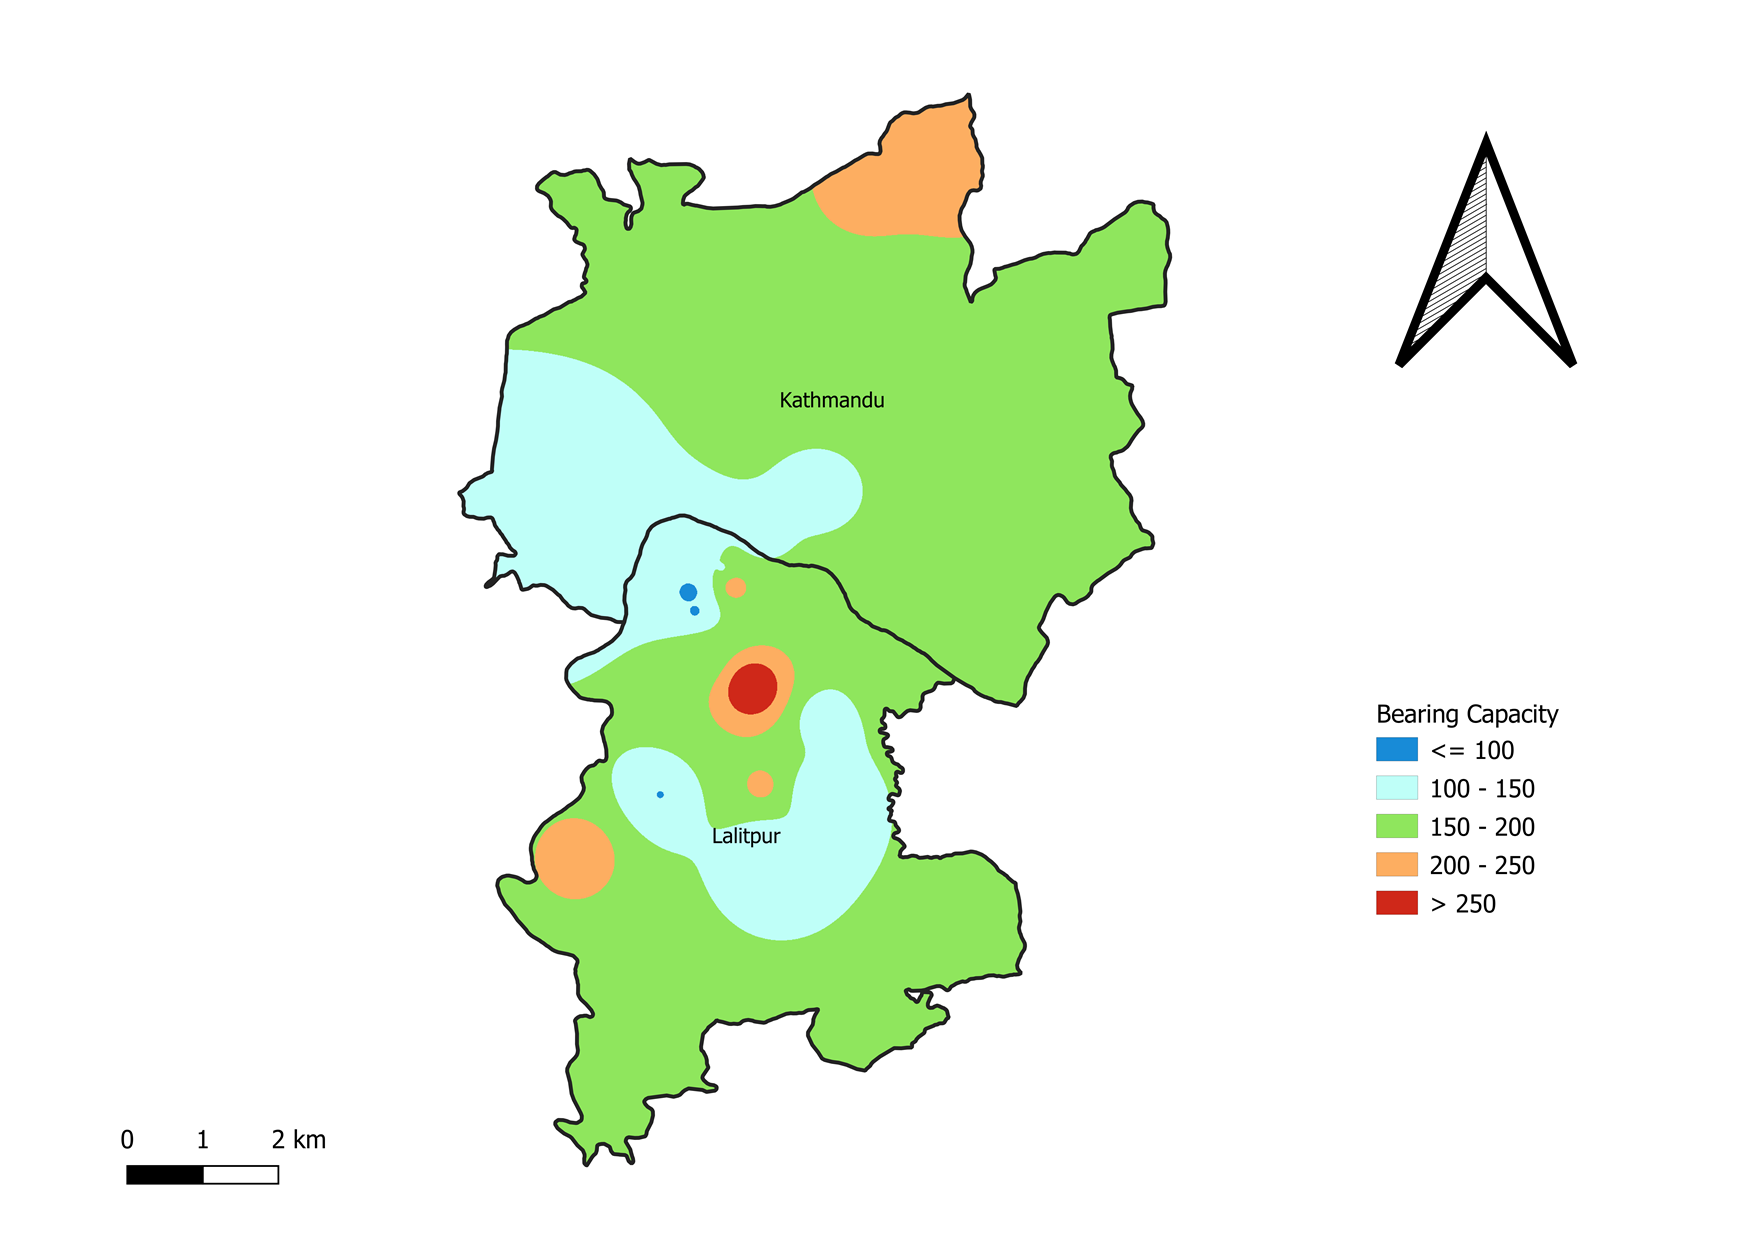
\includegraphics[width=\linewidth, height=\textheight,keepaspectratio]{in/map/Deflection_4_5.png}
\caption{BC at 4.5m depth}
\end{figure}
\pagebreak

\section{Liquefaction(LPI) Table}
\begin{table}[!h]
\caption{Liquefaction(LPI) Table}
\begin{tabularx}{\textwidth}{ | l | p{0.5\textwidth} | X | }
\hline
 \textbf{S.N.} & \textbf{Location} & \textbf{LPI}\\
\hline
 1 & Thapathali, Kathmandu & 26.184 \\
 2 & Anamnagar, Kathmandu & 18.597 \\
 3 & Bakhundol Lalitpur & 6.858 \\
 4 & Balkumari, Lalitpur & 16.423 \\
 5 & Bansbari, Kathmandu & 1.518 \\
 6 & Bhaisipati, Lalitpur & 0.045 \\
 7 & Gahanapokhari, Kathmandu & 0.670 \\
 8 & Mulpani, Kathamndu  & 1.325 \\
 9 & Itachhe tol, Bhaktapur & 0.479 \\
 10 & Jawalakhel, Lalitpur  & 0.743 \\
 11 & Jawalakhel & 12.442 \\
 12 & Tangal, Kathmandu & 4.132 \\
 13 & Harihar Bhavan, Lalitpur & 31.190 \\
 14 & Kuleswore, Kathmandu & 17.653 \\
 15 & Lainchour, Kathmandu & 1.319 \\
 16 & Tahachal, Kathmandu & 50.302 \\
 17 & Satdobato, Lalitpur & 0.383 \\
 18 & Naxal, Nagpokhari Kathmandu  & 1.661 \\
 19 & Mandikatar, Kathmandu  & 1.028 \\
 20 & Mandikhatar, Kathmandu  & 2.204 \\
 21 & Lainchaur, Kathmandu  & 4.616 \\
 22 & Kupondole, Lalitpur & 2.649 \\
 23 & Kupondole, Lalitpur & 10.705 \\
 24 & Khumaltar, Lalitpur & 16.796 \\
 25 & Khumaltar, Lalitpur  & 11.200 \\
 26 & Kalopul, Pumori, Kathmandu & 6.137 \\
 27 & Gwarkho, Lalitpur & 19.032 \\
 28 & Kumaripati, Lalitpur & 0.000 \\
 29 & Kupandole, Lalitpur & 20.590 \\
 30 & Thapathali & 4.920 \\
 31 & Kirtipur, Kathmandu & 8.512 \\
\hline
\multicolumn{2}{|X|}{\mbox{Mean($\overline{x}$)}} & 8.334  \\
\multicolumn{2}{|X|}{\mbox{Standard deviation($\sigma$)}} & 8.579 \\
\multicolumn{2}{|X|}{\mbox{Minimum($x_{min}$)}} & 0.000 \\
\multicolumn{2}{|X|}{\mbox{Maximum($x_{max}$)}} & 31.190 \\
\hline
\end{tabularx}

\end{table}
\pagebreak

\section{LPI\index{map}}
\begin{figure}[!hbt]
\centering
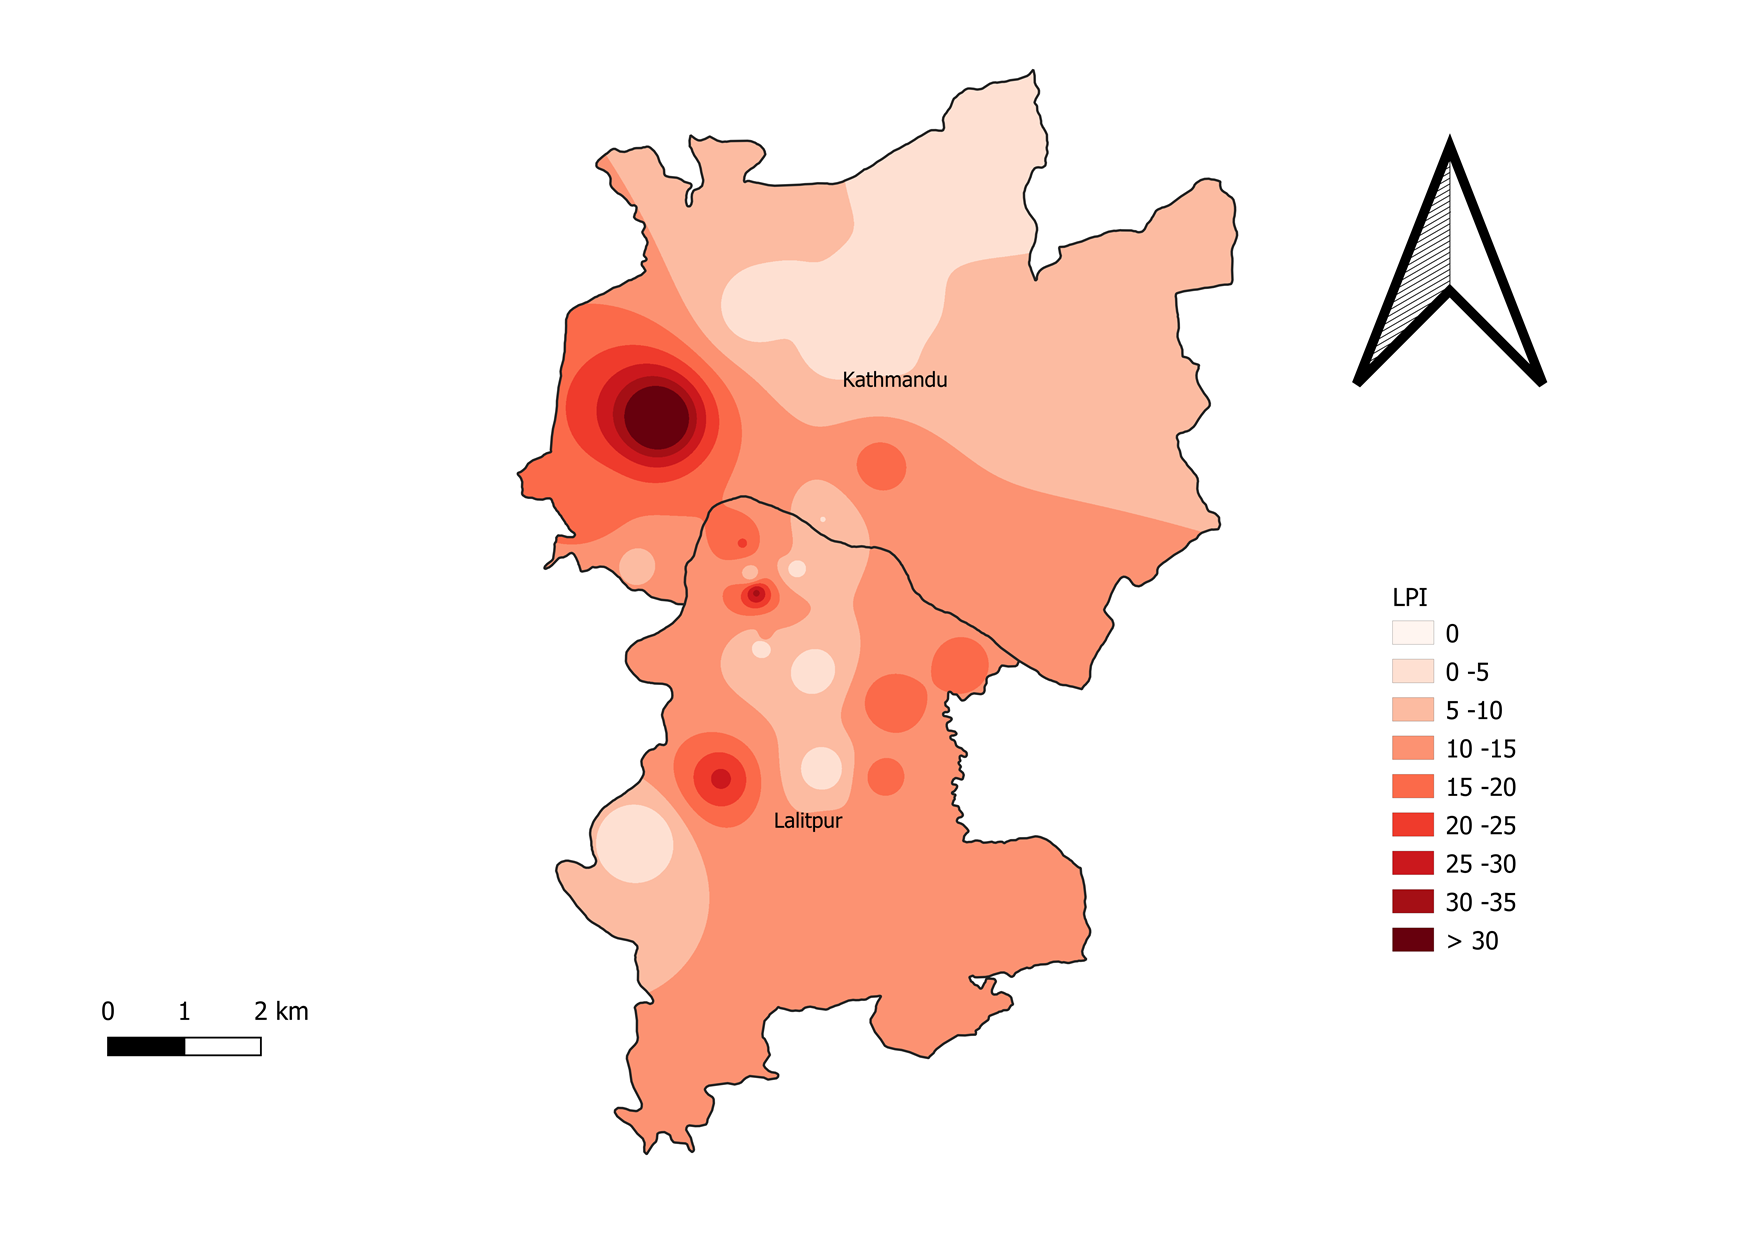
\includegraphics[width=\linewidth, height=\textheight,keepaspectratio]{in/map/lqi2.png}
\caption{LPI}
\end{figure}
\pagebreak